\documentclass[12pt,fleqn,reqno,letterpaper]{article}

\usepackage{float}
\usepackage{graphicx}
\usepackage{setspace}
\usepackage{textcomp}
\usepackage{fullpage}
\usepackage{url}
\usepackage[usenames,dvipsnames,svgnames,table]{xcolor}
\usepackage{longtable}
\usepackage[parfill]{parskip}
\usepackage[titletoc,title]{appendix}
\usepackage{hyperref}
%\usepackage{mdframed}  % not availble on ubuntu

% special math formatting
\usepackage{amsmath}

\bibliographystyle{IEEEtran}
\begin{document}
\begin{titlepage}
\begin{center}
  \textsc{\LARGE University of Waterloo}\\[0.5cm]
  \textsc{\Large E\&CE: 457B}\\[0.5cm]
  \vfill
  { \huge \bfseries Application of Expert System for Job Selection \\[0.4cm] }
  \vfill
  Group: 8 \\
  Garrett Everding \\
  Samuel Cheung \\
  Junwin Li

  \vfill
  \today
\end{center}
\end{titlepage}
\tableofcontents
\clearpage
\listoffigures
\clearpage
\listoftables
\clearpage

\begin{abstract}
Job selection for full-time employment is often a difficult decision due to a person’s preferences and factors associated with each job. An applicant may avoid a job that pays well because it requires a long commute to work, whereas another applicant may be indifferent to the commute. Common criteria considered when picking a job include salary, location, company reputation, company culture and job interest. An expert software system can help with job selection, so that time and effort on behalf of the user can be reduced.

An expert system can use fuzzy logic to take a set of inputs from a user to make decisions based on a set of rules. In the context of this problem, the expert system will determine what job is best suited based on the preferences of the user. Users will specify quality ranges for various criteria found in job postings. These ranges are mapped to linguistic hedges that are represented by membership functions within the universe of discourse of job happiness. Scalar job data from postings will be inputted into each membership function and evaluated. The system produces happiness values out of 100. A decision of the best job(s) is outputted based on the results of each membership function.

An illustrative example of a single criteria is given as follows: John believes that "\$60,000 salary per year is good".
\begin{itemize}
  \item The salary of \$60,000 is mapped to a membership function equalling "good"
  \item ABC Technologies has a job with salary posting of \$61,000 per year
  \item Given the membership function is adequate, \$61,000 per year will yield a high output
\end{itemize}
\end{abstract}
\nocite{FLS_MD,FLS_KD,FLS_ANN}


\clearpage
\section{Introduction}
A common problem facing students heading into the job market is deciding which job to apply for and what job to take.  The first job the new grad obtains will have great significant impact to their career path moving forward.  Looking through job descriptions, deciphering whether or not the job is suitable towards their needs and wants is a very time consuming process..  Advisors on job selection are often unavailable to students and are most likely not as reliable.  Though companies have Human Resource (HR) departments to provide guidance regarding the “fit” of a application, these advice may have biases towards the company.  The use of an expert system will improve the quality of jobs taken by new grads by improving the process of matching a new grads wants and needs to a set of possible jobs.

An expert system is a branch of artificial intelligence that is used to advise decisions based on input.  Our expert system will implement an artificial intelligence that advises students on what they should take, based on their preferences.  In order to emulate the decision making process of a human, fuzzy logic is used to implement the expert system.  The system will take inputs from the student.  These inputs are converted into membership functions, where then a database of company data is applied to each graph. A set of logical if-then rules, which are generated and then mapped to consequences that produces a happiness output.  This output determines a job that best matches the students inputs.

This expert system is autonomous and does not require human supervision to run.  This eliminates the necessity of a dedicated advisor since a machine is performing the work.  It can easily recreate the dialogue between an advisor and student and will hopefully produce selections of similar quality.  The expert system can be distributed through the use of a web interface.  A student can easily gain access to the system saving time and effort on their part.  The expert system is not only limited to students selecting jobs, but can be general enough to advise any candidate looking for a job.

\section{Background}
\subsection{Norm Operator Alternatives for Rules}
The norm operators are variable for the aggregation of inputs for each individual rule. This means that the inputs of rules can be merged differently, and thus the best-suited operator for each specific rule can be chosen for the most accurate inference of happiness. For example, one rule might relate salary and bonuses, which can reasonably be aggregated by the average of the inputs because they are similar and both have the same universe of discourse of money value. On the other hand, something such as company globalization and company reputation, may not necessarily have a consistent correlation to happiness in all scenarios, so the minimum of the inputs means the happiness is only as certain as the worst-case. The best-suited operator for a specific rule depends on the psychological aspects of the inputs to job happiness, historical background, and tweaking of our system.

A selection of operator alternatives considered for input aggregation is shown in Table \ref{tbl:INPUT-AGGREGATION} below. The formula in the table uses two variables (x and y) to represent the certainty of two input membership functions being aggregated.

\begin{table}[H]
  \caption{Norm Operator Alternatives for Rules}
  \label{tbl:INPUT-AGGREGATION}
  \centering
\begin{tabular}{|c|l|l|}
\hline
\textbf{Input Aggregation Operator} & \textbf{Additional Parameters} & \textbf{Formula}                                      \\ \hline
Min                                 &                                & $\text{min}(x,y)$                                     \\ \hline
Max                                 &                                & $\text{max}(x,y)$                                     \\ \hline
AlgebraicProduct                    &                                & $x \times y$                                          \\ \hline
ArithmeticMean                      &                                & $\frac{(x+y)}{2}$                                 \\ \hline%
FuzzyAnd                            & $\text{Weight} = p (0-1)$      & $(1-p) \times min(x,y) + p \times \frac{(x+y)}{2}$ \\ \hline
EinsteinProduct                     &                                & $\frac{(x \times y)}{(1 + (1 - x)\times(1-y))}$       \\ \hline
\end{tabular}
\end{table}

Minimum is an operator that is used in practice for neural networks \cite{FAKHRI}. It works well because it helps eliminate rules with no intersection with a linguistic hedge, such as a minimum wage job with the rule “If pay is high (>\$120,000) and bonus is high (>\$20,000) then happiness is high”. The intersection of the minimum wage pay and fuzzy high pay will have no intersection, thus the aggregate will be zero certainty of high happiness.

Maximum is very inapplicable because there is a large rule set for job happiness. Each of the inputs in a rule require consideration to account for lowered happiness.

The remaining operators add some depth to the certainty of happiness. They make sense that they aggregate based on the values of all input membership functions for a given rule, rather than just taking the minimum or maximum.

The best aggregation norm operator depends on the relation between the inputs for a given rule. From our research on the psychological background and testing of our expert system, the minimum (Min) operator appeared to be a reasonable operator for the baseline for all of our rules.

\subsection{Norm Operator Alternatives for Final Output}
The norm operator for the combining of all rule outputs can also be changed, but only one can be selected for the whole system. There are very many possible norm operators, but only a selection of them were considered. The alternatives considered are in Table \ref{tbl:FINAL-NORM} below. The formula in the table uses two variables (x and y) to represent the certainty of two membership functions.

\begin{table}[h]
\caption{Nprm Operator Alternatives for Final Output}
\label{tbl:FINAL-NORM}
\centering
\begin{tabular}{|c|c|}
\hline
\textbf{Norm Operator} & \textbf{Formula}  \\ \hline
Max                    & max(x, y)         \\ \hline
BoundedSum             & max(1, x+y)       \\ \hline
ArithmeticMean         & $\frac{(x+y)}{2}$ \\ \hline
\end{tabular}
\end{table}

Maximum operator is a common choice for joining rule outputs [FAKHRI]. In English, it takes the maximum certainty of happiness from each linguistic hedge, and uses that as the inferenced output. This is reasonable because the rules used consider the significant and important aspects of job happiness. This means that whichever rules create the most certainty for happiness for each linguistic hedge, will be the standout factor for the final job happiness. The maximum operator also ignores rules that do not create any certainty of happiness, i.e. there is intersection of a rule input.

The bounded sum operator is the second option with a slightly different theory than the standout factor theory used for the maximum operator. In bounded sum, the theory is that many factors of happiness or unhappiness lead to a greater chance of happiness. Users will always have different preferences, so happiness for one factor may not be the same for everyone. This operator leverages disjunction probability by considering that if there is some certainty of happiness for multiple factors (rules), then it is more certain that the user will be happy or unhappy for at least one of these factors. The problem with this is that the expert system can easily have very many rules, and as a result, the sum of all the rule outputs will lead to a final output of 100\% certainty for all happiness. This can be easily alleviated by putting a weight for each rule (max(1,0.5(x+y))), such as weight = 1/(number of rules).

The arithmetic mean, or average, operator can be troublesome if there are very many rules, and many of them have zero or low happiness certainty. These low values would unnecessarily lower the average of the final output happiness.

From the analysis and reasoning of of the operators, the maximum (Max) operator appeared to be a reasonable operator for the baseline of all of our rules.

\subsection{Defuzzification}
Defuzzification is important for interpreting, accurately, the expected job happiness. The options considered were centroid (center of gravity), left maxima, right maxima, and mean of maxima. Looking at only the maxima certainty is not reasonable because this completely neglects the factors creating the area of the inferenced happiness function that is less than the maximum certainty. All ranges of inferenced happiness needs to be considered, and thus centroid was chosen as the best alternative.

\section{Tools}
Our expert system is based on the pyfuzzy framework \cite{pyfuzzy}. The 2D graphs and 3D graphs are generated using gnuplot \cite{gnu-plot}.

\section{Design Overview}
The purpose of our system is to select the optimal job for a user based on their preferences. To accomplish this, the system takes input from a user regarding their preferences relating to the various aspects of a potential job and selects the job that will result in the user being the happiest. This is accomplished through the application of fuzzy logic to construct a expert system. Figure \ref{fig:block-diagram} provides a high level architecture for our expert system. The operations used as our baseline for each step is shown in brackets. The inputs of rules are aggregated using minimum, the final output is inferenced using maximum, and lastly the defuzzification of the happiness value is done using center of gravity.

\begin{figure}[H]
  \centering
  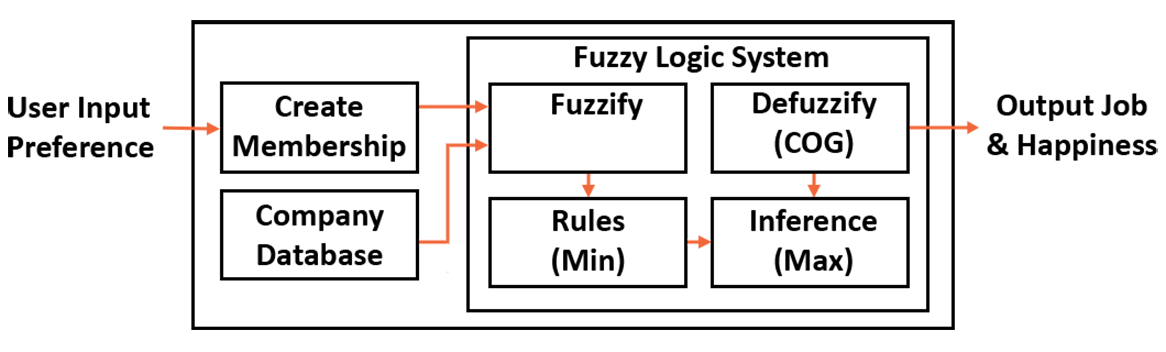
\includegraphics[scale=0.3,natwidth=1166,natheight=352]{fig/BLOCK_DIAGRAM.png}
  \caption{System Block Diagram}
  \label{fig:block-diagram}
\end{figure}

The flow of information through our system starts with collection of user input. The user’s preferences are then fed into the fuzzy logic controller which builds a set of membership functions representing the user’s preferences. These membership functions are then combined with a prebuilt rule set. The shape of the membership functions and set of rules are based on research from studies in the areas of employee happiness and engagement in the workforce. Once this has been completed, the happiness for each potential job is computed and the top 3 jobs are presented to the user.

\subsection{Inputs}
For our initial prototype the system allows users to specify their preferences for salary, company size and reputation. These selected inputs are a subset of all possible inputs as there are numerous inputs that our system could take [ref; Job Satisfaction] to aid in the selection of the optimal job. These specific inputs were chosen for our initial implementation because they are unique to each individual and they are all factors that have crisp values from the perspective of employer.

From the perspective of the user, they specify a set of possible ranges for the given inputs (salary, company size and reputation). For each input, the user provides a range of values for each linguistic hedge. The linguistic hedges are defined ahead of time for each input. Table \ref{tbl:LINGUISTIC-HEDGES} outlines the linguistic hedges for each input.


\begin{table}[h]
  \caption{Linguistic Hedges for Baseline Inputs}
  \label{tbl:LINGUISTIC-HEDGES}
  \centering
\begin{tabular}{|l|l|}
\hline
\textbf{Input} & \textbf{Linguistic Hedges} \\ \hline
Salary         & Bad, Okay, Good            \\ \hline
Company Size   & Small, Medium, Large       \\ \hline
Reputation     & Unnoticed, Noticed         \\ \hline
\end{tabular}
\end{table}

In the case of salary from Table \ref{tbl:LINGUISTIC-HEDGES}, a user inputs a range of salaries that they consider low, another range that they consider okay and finally a range of salaries that they consider good. The set of inputs are then fed into the fuzzy logic system to generate the appropriate membership functions.

\subsection{Membership Functions}
\label{sec:membership_fn}
For the initial implementation our system used Trapezoid membership functions for each input. The Trapezoid membership function was chosen because it modeled the inputs accurately given the fact that each input from Table \ref{tbl:LINGUISTIC-HEDGES} allows the user to specify a range of values for each linguistic hedge. Therefore, in between the high and low value, the user is 100\% certain that ranges of values maps to that linguistic hedge. However, outside that range the user is less certain. This is where the fuzziness comes into play in the system. Example membership functions for pay, company size and reputation are given in Figure \ref{fig:BPM}, Figure \ref{fig:BEM} and Figure \ref{fig:BRM} respectively. These membership functions were generated using one of our test users.

\begin{figure}[H]
  \centering
  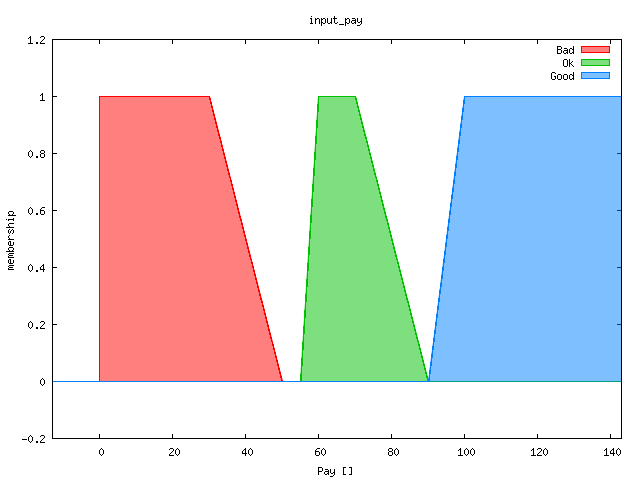
\includegraphics[scale=0.5,natwidth=640,natheight=480]{fig/baseline_input_pay.png}
  \caption{Membership functions for Bad, Okay and Good Pay}
  \label{fig:BPM}
\end{figure}
\begin{figure}[H]
  \centering
  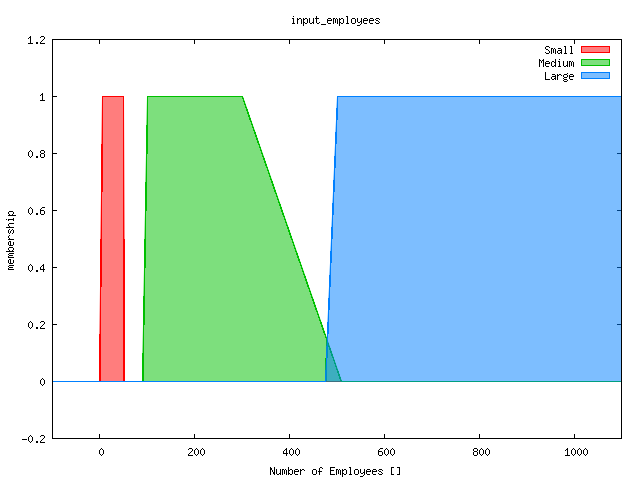
\includegraphics[scale=0.5,natwidth=640,natheight=480]{fig/baseline_input_employees.png}
  \caption{Membership functions for Small, Medium and Large Companies}
  \label{fig:BEM}
\end{figure}
\begin{figure}[H]
  \centering
  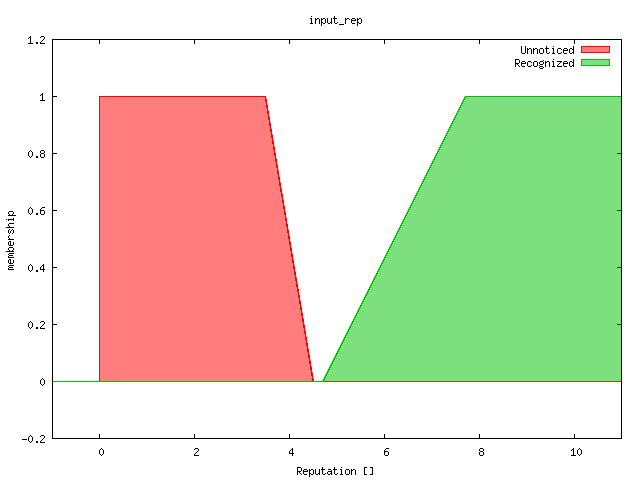
\includegraphics[scale=0.5,natwidth=640,natheight=480]{fig/baseline_input_rep.png}
  \caption{Membership Functions for Unnoticed and Noticed Reputation}
  \label{fig:BRM}
\end{figure}

For each of the membership functions in the initial implementation, there is no guarantee that they will overlap. An example of this occurring can be found in Figure BPM. The user preferences that generated this membership function can be found in Table \ref{tbl:USER-PAY-PREF}.

\begin{table}[H]
  \caption{Example User’s Preferences for Pay}
  \label{tbl:USER-PAY-PREF}
  \centering
\begin{tabular}{|l|l|l|}
\hline
\textbf{Linguistic Hedge} & \textbf{Low} & \textbf{High} \\ \hline
Bad                       & 0            & 30000         \\ \hline
Okay                      & 60000        & 70000         \\ \hline
Good                      & 100000       & 130,00        \\ \hline
\end{tabular}
\end{table}
To construct the membership function in Figure BPM, the system uses the low and high values as the end points for the rectangular portion of the trapezoid. The left and right and portions of the trapezoid are then calculated independently. In the case of the left hand side of the low and okay pay membership function the system assumes that a pay lower than the lower bound is always less preferred. For the right hand side of the low and okay pay membership functions, the system uses the heuristic that as pay increases past the high bound an increase in salary of \$5,000 is not as significant so it probably still belongs in the okay universe of discourse. High pay uses a similar heuristic; a salary of \$5,000 or \$10,000 less than the lower bound is not significant enough to remove it from the universe of discourse. This results is a shallow slope for both the right hand side of the low and okay membership functions and the left hand side of the good membership function.

\subsection{Rules}
The rules for the system are static in the sense that they are defined ahead of time and are not configurable by the user or employer. Additionally, each rule only combines 2 inputs to the system. This results in a larger set of rules that are easier to read and reason about. Using the same user and membership function from Section \ref{sec:membership_fn} and the rules for the system the happiness can be graphed as a function of the inputs. The happiness as a function of pay and number of employees can be seen in Figure \ref{fig:PE}. Happiness as a function of reputation and number of employees can be seen in Figure \ref{fig:RE}. Finally, happiness as a function of reputation and pay can be seen in Figure RP.

\begin{figure}[H]
  \centering
  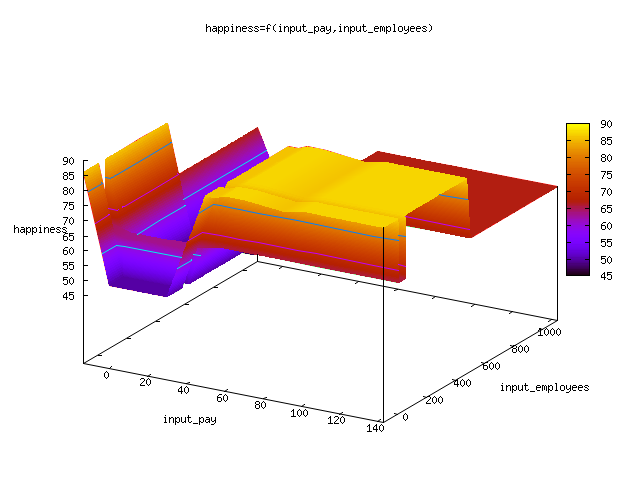
\includegraphics[scale=0.5,natwidth=640,natheight=480]{fig/baseline_input_pay_input_employees_happiness.png}
  \caption{Employee Happiness as it relates to Pay and Company Size}
  \label{fig:PE}
\end{figure}

\begin{figure}[H]
  \centering
  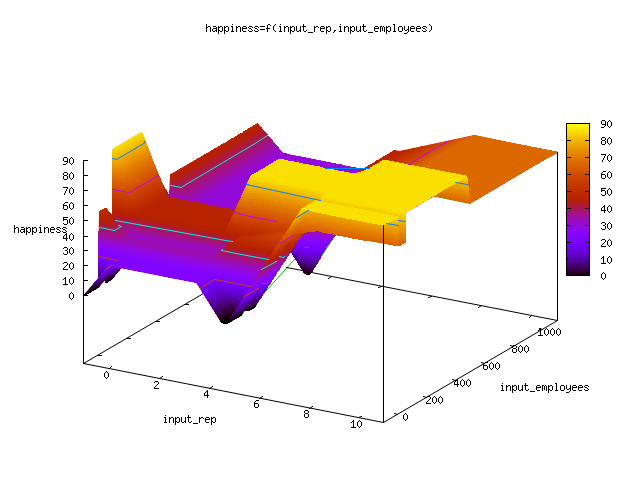
\includegraphics[scale=0.5,natwidth=640,natheight=480]{fig/baseline_input_rep_input_employees_happiness.png}
  \caption{Employee Happiness as it relates to Reputation and Company Size}
  \label{fig:RE}
\end{figure}

\begin{figure}[H]
  \centering
  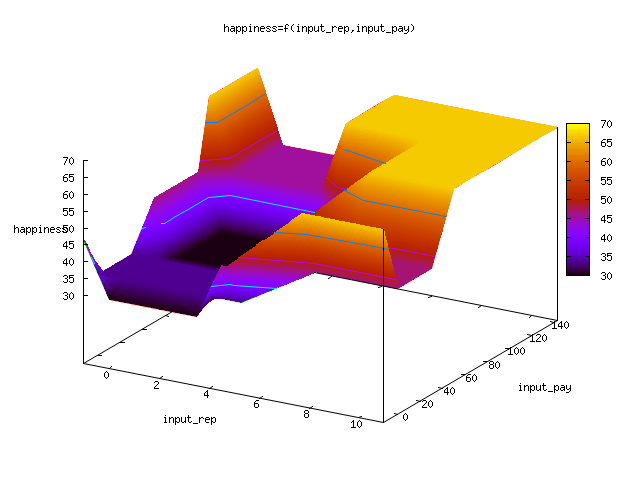
\includegraphics[scale=0.5,natwidth=640,natheight=480]{fig/baseline_input_rep_input_pay_happiness.png}
  \caption{Employee Happiness as it relates to Reputation and Pay}
  \label{fig:RP}
\end{figure}

The base set of rules for the system are based on studies looking at factors affecting employee engagement and personal preferences of colleges.

\subsection{Happiness}
\label{sec:happiness}

Happiness is defined in terms of 3 linguistic hedges; bad, medium and good. The membership function for happiness is provided in Figure \ref{fig:HAPPINESS-MF}.

\begin{figure}[H]
  \centering
  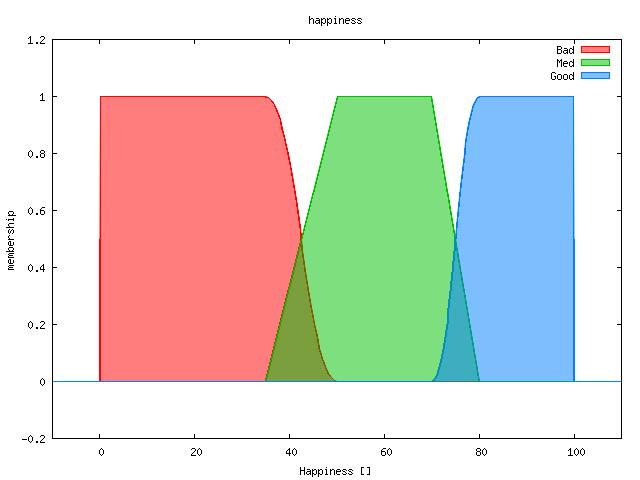
\includegraphics[scale=0.5,natwidth=640,natheight=480]{fig/happiness.png}
  \caption{Happiness Membership Functions}
  \label{fig:HAPPINESS-MF}
\end{figure}

The process of defuzzification is performed using center of gravity (COG) function for each job in our job database from Figure \ref{fig:block-diagram}.

\subsection{Scalability}
With fuzzy systems, the amount of computation required for rule inference and output inference depends on the number of rules and segment size used for the calculation. Each rule requires operators performed on the inputs, and then an additional operator performed when merging into the final inferenced output. Segment size is the spacing between points used for calculations; it is the precision for the calculation. A smaller segment size means more computations required for the 0-100 domain of happiness. Our system uses a segment size of 0.5 for most calculations.

For our expert system, it also generates a happiness value for every company in our company database in order to find the top 3 jobs for the user specified input.

\subsection{Summary of Design Overview}
This is the base application with a minimal set of inputs and rules to test the functionality of the system. The following sections add onto this implementation by increasing granularity and adding an additional input into the expert system.

\section{Design Improvement: Granularity}
The granularity implementation of the expert job selection system involves adding membership functions to each input that map in between existing membership functions.  The purpose of this implementation is to determine whether a greater number of linguistic hedges for a given input improves accuracy of the system when selecting an optimal job for a given user.  These additional membership functions provide more fuzziness and a greater degree of configurability in the rule set.

\subsection{Implementation}
In order for the datasets provided by the user to be compatible with the granularity implementation, the in between membership functions are calculated rather than inputted by the user.  The shape of the membership functions are similar to existing membership functions.  Most membership function will use the triangle function.  This shape was chosen to compliment the trapezoid function and maintain computation simplicity.  Further experimentation can be implemented in modifying the transition curve depending on how the user perceives the value of money, reputation and employee size.  To guarantee fuzziness between membership functions, the in between triangle functions are calculated such that the ends of the function are always overlapped with the slopes of the trapezoid functions.  This differs from the baseline implementation which allows for gaps between membership functions.  Though the option exist for calculated in between functions not to overlap, it was decided that overlapping membership functions would produce better output.  The use of overlapping membership functions guarantees fuzziness for inputs that land in between linguistic hedges.  Using any of the measure of fuzziness show that having overlap produces more fuzziness in the system, since a greater area of function is calculated.  The use of the triangle shape also ensure that calculated in between membership functions do not contribute greatly for situations where inputted membership functions are far away.  If a large gap were to occur between two membership functions, the slope of the in between membership function would be very broad, giving less weight to the output if an input were to occur on the in between membership function.

\begin{figure}[H]
  \centering
  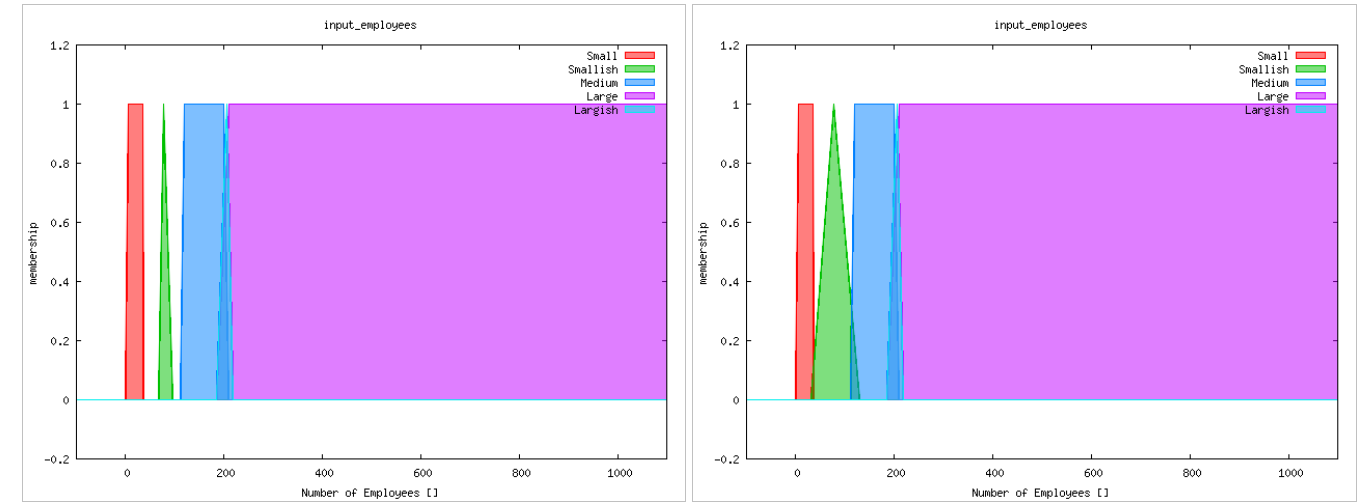
\includegraphics[scale=0.5,natwidth=1360,natheight=504]{fig/crossover.png}
  \caption{On left smallish(green) does not overlap where on right smallish does}
  \label{fig:CROSSOVER}
\end{figure}

To account for membership functions close together management of the in between membership functions must be implemented.  If membership functions already overlap having calculated membership function will decrease the overall fuzziness of the input.

\begin{figure}[H]
  \centering
  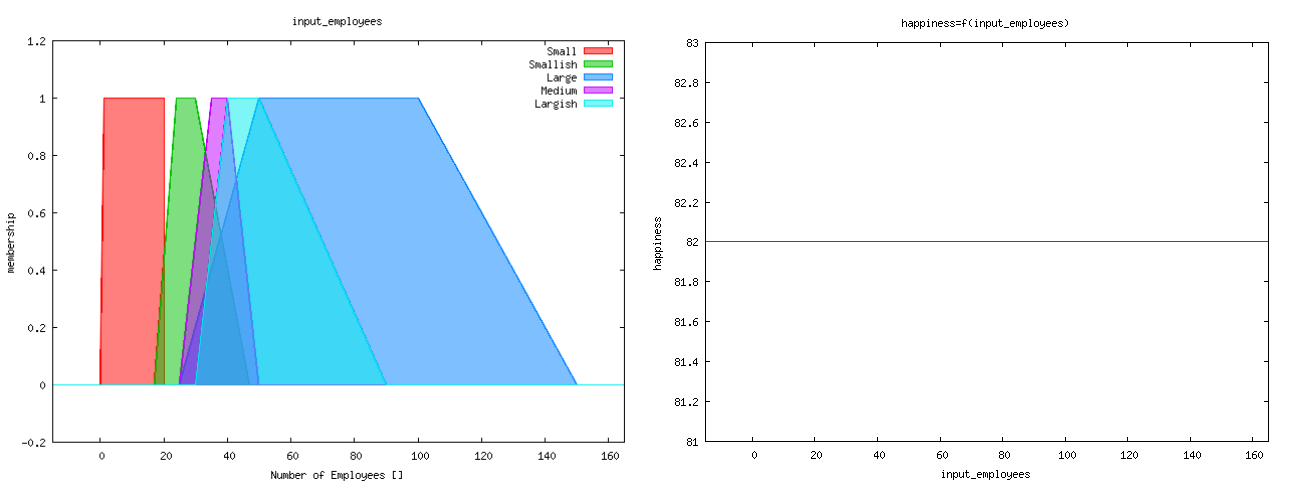
\includegraphics[scale=0.5,natwidth=1297,natheight=501]{fig/overlap.png}
  \caption{A closely overlapped function(Left) with its happiness output(Right)}
  \label{fig:OVERLAP}
\end{figure}

Figure \ref{fig:OVERLAP} shows an early implementation of the calculated in between membership functions.  With member functions so close together a constant happiness output is produced (The above happiness graph in Figure OVERLAP is a combination of all rules applied to the output as plotted along the number of employee inputs).  In order to avoid outputs such as Figure OVERLAP, the triangle membership function is manipulated to account for this.  The use of a triangle membership function minimizes the amount of overlap at the peak of the function.  If the ends of two membership functions are overlapped in such a way that the triangle membership function is encased in both of the two adjacent membership function, then the triangle membership function is not calculated.

Special interest is given to the reputation input and its calculated membership function.  The initial implementation of the reputation membership function had only two membership functions to represent good and bad reputation.  To account for a larger variety of rules, rather than implementing a static triangle function where the peak sits between the middle of the two ends of the membership functions, a skew is implemented instead.

\begin{figure}[H]
  \centering
  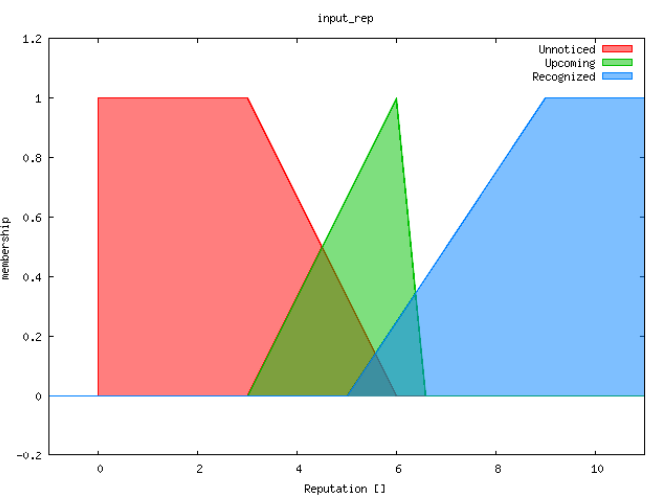
\includegraphics[scale=0.5,natwidth=656,natheight=501]{fig/upcoming_skew.png}
  \caption{Added upcoming linguistic hedge for reputation}
  \label{fig:UPCOMING-SKEW}
\end{figure}

This skew is shifted to the right, where the left slope is smaller than the right slope.  This represents the slow rise of reputation and a sharp decrease when transitioning to a recognized company.  As such, the linguist hedge associated with this membership function is mapped to the linguistic of “Upcoming”, as to represent up and coming companies.

\subsection{Rule Implementation}
With an increase in granularity, new rules are needed to extend the current behaviour of the ruleset and to produce new behaviour.  The new rules follow the same format of comparison between two inputs to produce a single happiness output.  To extend the rule sets for each granularity, all old rules need to be analyzed and re-implemented with similar behaviour.  Missing granularity rules will cause empty spaces within happiness output.

\begin{figure}[H]
  \centering
  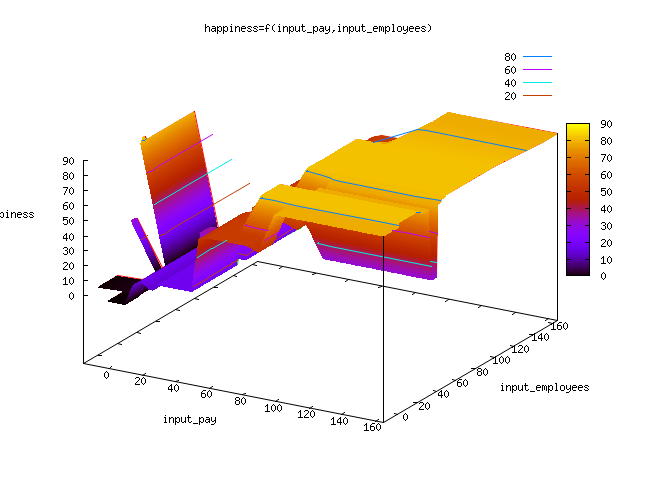
\includegraphics[scale=0.5,natwidth=650,natheight=501]{fig/extend_gran.png}
  \caption{Unextended ruleset for pay and employee size}
  \label{fig:EXTEND-GRAN}
\end{figure}
Figure \ref{fig:EXTEND-GRAN} shows the “smallish” for employee (15 - 35) input to have dropped happiness where it should be constant across all of high pay (>\$100,000).  The extended ruleset adds the missing granularity rules to keep the behaviour of the system constant.

To take advantage of the granularity, new rules are implemented to produce new behaviour in the system.  A variety of research was done to take advantage of this \cite{GRAN-2}.  A notable example of this is the change of happiness with respect to pay.  A study by Princeton showed that it was not the amount of money that made someone happy, but rather the lack of money that would make a person sad \cite{GRAN-1}.  With this in mind, new granularity can be used to represent this.

\begin{figure}[H]
  \centering
  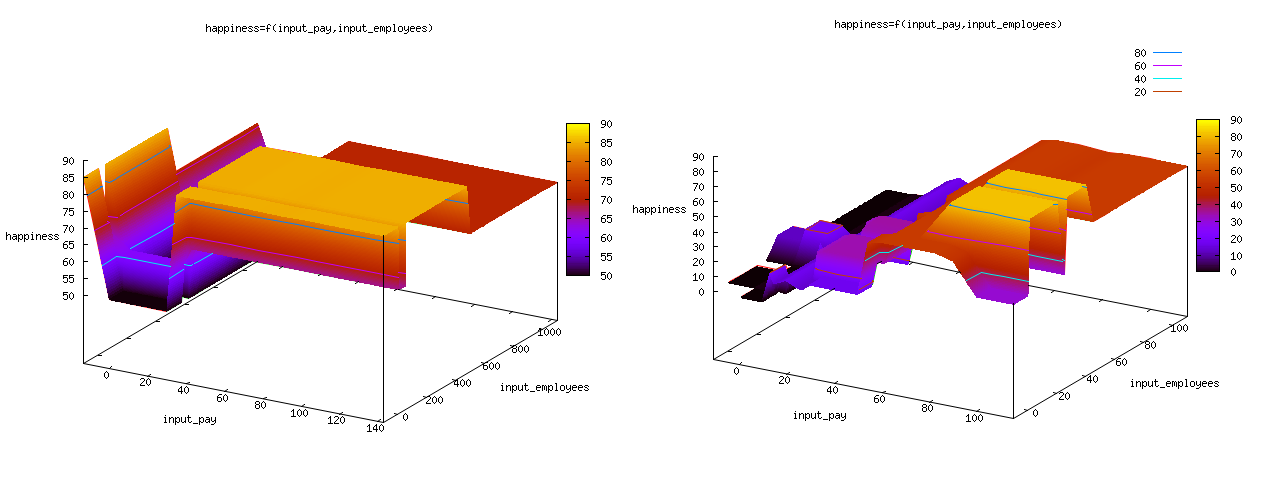
\includegraphics[scale=0.5,natwidth=650,natheight=501]{fig/new_gran_rule.png}
  \caption{Baseline(Left) and Granularity(Right) output of pay and company size}
  \label{fig:NEW-GRAN-RULE}
\end{figure}

Figure \ref{fig:NEW-GRAN-RULE} shows the baseline implementation and granularity implementation of pay versus employee size.  Comparing high pay and large companies happiness output, a slightly lower happiness is possible along with a slow decreasing happiness with granularity, whereas the baseline cannot do this.  The baseline assumes that all decent pay is good for small companies but granularity slowly degrades this.

\subsection{Summary of Granularity Design}
Observing output of the membership functions, an analysis of how granularity affects the output happiness function can be performed.  When membership functions are close together, the managed granularity functions do not affect the output due to enough fuzziness existing between the two membership functions.  When membership functions are far apart, the calculated membership function cause some level of output to be produced due to the in between membership function overlapping with the other membership functions.  Blank empty areas on the input graph that once did not produce any output now have a small amount of output.  This combined with the new ruleset have shown to give better performance in terms of accuracy.  Running tests against the same parameters as the baseline input, it was found that the granularity implementation showed to be 22\% more accurate over the original 11\% of the baseline.

For the given amount of performance increase there are great number of implementation details that need to be accounted for.  It was noticed that approximately 10 rules were implemented for the baseline implementation.  To account for the extension of rules and new behavioural rule, a total of 40 rules were needed for the granularity implementation.  If additional inputs were to be added the number of rules would vastly increase, which in turn would greatly increase the amount of time needed to implement each rule.  For the granularity analysis, only the implementation time for the rule set is considered rather than the computation complexity of rules during runtime.  Considering that even though the ruleset increases exponential to the number of inputs, a designer needs to approve and implement each rule.  The amount of rules added to the system is bounded by the amount a designer approves of.  For the amount of performance increase gained, the implementation time may not be justifiable due to the large increase in ruleset.  This however varies pending on whether or not a ruleset can cover all manner of logic for the given number of inputs.  In terms of overall performance the granularity has shown to be an overall improvement over the baseline.

\nocite{GRAN-3,GRAN-4}

\section{Design Improvement: Variety}
A fuzzy system is limited in improvement for a given set of inputs.  To improve the expert system, additional inputs are considered. Certainty aspect to rule inferencing is also considered for improvements. These changes are discussed in the following subsections.

\subsection{Additional Criteria}
Experimentation with changes to the happiness values and job selection results after adding a commute time criteria were performed. This added the following commute time linguistic hedges for user input: close, medium, and far. Only three trivial rules were added: \\
\begin{itemize}
\item If commute time is close, then happiness is high
\item If commute time is medium, then happiness is medium
\item If commute time is far, then happiness is low
\end{itemize}

Commute time is a factor considered by many people when selecting a job, and people often talk about their commutes to work. In the baseline, commute time is neglected, making some jobs appear to have high happiness value even though the commute time is over one and a half hours one-way.  The system was tested  against a user, with somewhat average preference on commute time, who specifies commute time as: close = 10 minutes, medium = 40 minutes, and far = 70 minutes to see the change in happiness values. The results of some selected jobs can be seen in Table \ref{tbl:DISTANCE-DIFF} below.

\begin{table}[h]
  \caption{Difference in Happiness After Considering Commute Time}
  \label{tbl:DISTANCE-DIFF}
  \centering
\begin{tabular}{|p{2cm}|p{4cm}|p{4cm}|p{4cm}|}
\hline
\textbf{Job Identification} & \textbf{Commute Time (minutes)} & \textbf{Happiness without Commute Time Rules (/100)} & \textbf{Happiness with Commute Time Rules (/100)} \\ \hline
1                           & 120                             & 71.73                                                & 49.27                                             \\ \hline
2                           & 60                              & 76.74                                                & 69.95                                             \\ \hline
3                           & 30                              & 86.98                                                & 86.1                                              \\ \hline
4                           & 5                               & 75.87                                                & 82.52                                             \\ \hline
\end{tabular}
\end{table}
Clearly, job number one had a significant decrease in job happiness. It appeared as a job with decent happiness, to a job that probably should not be considered by the user. It is also important to note that a user that is more tolerable to longer commutes would not be as impacted by the new commute time rules. The following figures show the final inferenced happiness of job number one without considering commute time and after considering commute time.

\begin{figure}[H]
  \centering
  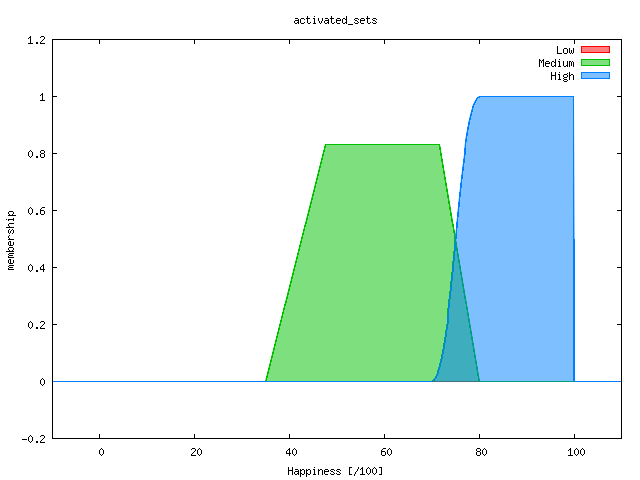
\includegraphics[scale=0.5,natwidth=640,natheight=480]{fig/NO_COMMUTE.png}
  \caption{Happiness Membership Function without Commute Rules}
  \label{fig:NO-COMMUTE}
\end{figure}
\begin{figure}[H]
  \centering
  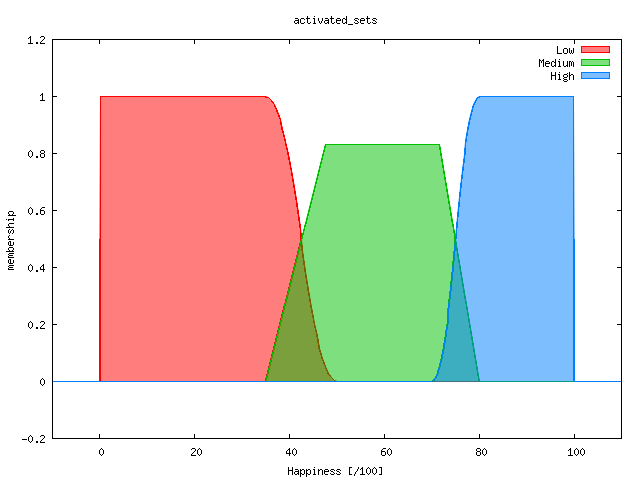
\includegraphics[scale=0.5,natwidth=640,natheight=480]{fig/YES_COMMUTE.png}
  \caption{Happiness Membership Function with Commute Rules}
  \label{fig:YES-COMMUTE}
\end{figure}

Looking at happiness, it is trivial that longer commutes lead to less happiness, in general. It is important to ensure the system accounts for new inputs and new rules in job happiness. This analysis shows that adding new rules do play an important role for the expert system in determining job happiness. There is very many criteria for jobs, and many of which play factors in job happiness. Adding more criteria/inputs, along with accurate rules that correlate them to happiness, result in a better system.

\subsection{Certainty of Rules}
The certainty of a rule output can be altered for a more accurate final inferenced happiness. The purpose for doing this is to modify the expected correlation of a rule to happiness because the accuracy of rules is very subjective depending on the user. Certainty can be applied to rules separately. One rule may have more influence on a user’s happiness over another. As an additional improvement to account for this, after the rule output is inferenced, an additional step can be applied to the membership function using a certainty value (0-1) and a norm operator. The operators we considered were only minimum and algebraic product.

Looking at happiness, it is trivial that longer commutes lead to less happiness, in general. It is important to ensure the system accounts for new inputs and new rules in job happiness. This analysis shows that adding new rules do play an important role for the expert system in determining job happiness. There is very many criteria for jobs, and many of which play factors in job happiness. Adding more criteria/inputs, along with accurate rules that correlate them to happiness, result in a better system.Tests were done with certainty values of 0.7 for rules that were less certain to be accurate, such as “If company size is small and reputation is high, then happiness is high.” Good reputation leads to higher happiness, but company size is not always a correlating factor to happiness. Rules that were more certain were kept at 1 certainty, to have no change from the baseline. This change did not change the happiness values much since the final inference is done using the maximum. However, there was a slightly lowered score for a job that had criteria matching a couple of the rules with lowered certainty. Certainty has a stronger effect when changing the norm operator used for final inferencing, as discussed in the following section.

\subsection{Modifications}
As the number of inputs increases, the number of rules will increase as well. This means that it becomes more likely that a happiness linguistic hedge will be at 100\% certainty. This is a problem if we get the final inferenced happiness via the max of the rule outputs, which is done in the baseline. If some or all of the linguistic hedges are often at 100\% certainty, then the defuzzification of job happiness values becomes very similar for many jobs. This makes it harder to differentiate between job happiness and job selection, and it also lowers the accuracy of the output job happiness.

To combat this problem with the maximum operator for the system when adding more inputs and rules, the final output inference operator can be changed. Arithmetic mean (average), as discussed in a previous section, seems like a feasible formula we can base an improved formula on. As mentioned previously, the problem is that some rules produce 0 certainty and may skew the results. This can be alleviated by only including rules that have at least some aggregated happiness output in the final output average.

For all input membership functions, it also becomes mandatory to have a certainty value for every value in the specified universe of discourse range. For example, pay is limited to \$0 to \$200,000 and every salary value should be covered by at least one membership function (any certainty). This is because if there is no value for a given salary, then for a job with that given salary, all rules that incorporate pay is voided since there is no intersection to create an inferenced happiness function for that rule (when operators such as minimum to aggregate inputs). An example would be to create membership functions that match high and low of neighbouring linguistic hedges, as shown in Figure \ref{fig:HIDE-GAPS} below.

\begin{figure}[H]
  \centering
  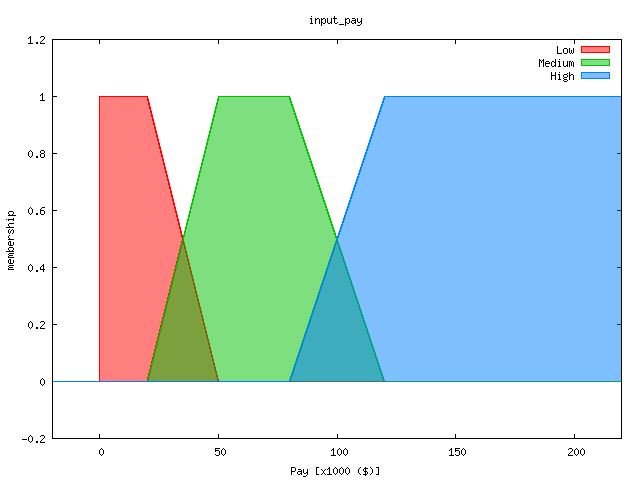
\includegraphics[scale=0.5,natwidth=640,natheight=480]{fig/HIDE_GAPS.png}
  \caption{Generated Membership Function with Complete Coverage}
  \label{fig:HIDE-GAPS}
\end{figure}

\section{Results}
\subsection{Execution Times}
The execution time for varying rules and jobs can be seen in Table \ref{tbl:EXECUTION-TIMES} below. The tests were performed on a machine with an Intel i5-4600M with 8 GB of RAM.

\begin{table}[h]
  \caption{Execution Times for Varying Number of Rules and Companies}
  \label{tbl:EXECUTION-TIMES}
  \centering
\begin{tabular}{|p{7cm}|p{3.5cm}|p{5.5cm}|}
\hline
\textbf{Number of Rules (2 inputs each)} & \textbf{Number of Jobs} & \textbf{Execution Time (seconds)} \\ \hline
10                                       & 20                      & 0.090s                            \\ \hline
20                                       & 20                      & 0.095s                            \\ \hline
30                                       & 20                      & 0.104s                            \\ \hline
40                                       & 30                      & 0.119s                            \\ \hline
40                                       & 40                      & 0.129s                            \\ \hline
40                                       & 50                      & 0.137s                            \\ \hline
\end{tabular}
\end{table}

It can be seen that the computation is very fast, considering it is done in Python. The number of jobs is not expected to grow very large for user in a given area. Also, the number of rules will continue to grow, but only adds a negligible amount of additional time. This should be fine since job selection is not high demand and very frequent activity people do.

\subsection{Correctness}
Testing each implementation of the system was done with a selection of people.  While the user was inputting data to the system, they were also asked which choice of job within the database he/she would pick.  The user’s data would be run against the system and the highest happiness output is displayed to the user.  If multiple jobs tie or show to be close in score, the jobs are pushed into a queue and selected at random. This output is compared against what the user expected to select.  Table \ref{tbl:INIT-RESULTS} shows the initial results when a single job is picked.

\begin{table}[h]
  \caption{Correctness of Expert System when Selecting One Job}
    \label{tbl:INIT-RESULTS}
    \centering
\begin{tabular}{|l|l|l|l|}
\hline
                            & \textbf{Baseline} & \textbf{Granularity} & \textbf{Variety} \\ \hline
\textbf{Percentage correct} & 11.11\%           & 33.33\%              & 11.11\%          \\ \hline
\end{tabular}
\end{table}

Observing Table \ref{tbl:INIT-RESULTS}, the expert job selection system has shown to be poor at selecting the expected job.  An analysis on the system was done to determine why these results were occurring.  It was found that rather than producing the top expected job, the system would encompass the top expected job within its top three results.  When checked if the expected result was contained within the top three results returned by the system a great improvement was found.

\begin{table}[h]
  \caption{Correctness of Expert System when Selecting Top Three Jobs}
    \label{tbl:IMPROVE-RESULTS}
    \centering
\begin{tabular}{|l|l|l|l|}
\hline
                            & \textbf{Baseline} & \textbf{Granularity} & \textbf{Variety} \\ \hline
\textbf{Percentage correct} & 11.11\%           & 33.33\%              & 11.11\%          \\ \hline
\end{tabular}
\end{table}

Table \ref{tbl:IMPROVE-RESULTS} show an overall improvement to the system.  Of the three implementations, granularity has shown to perform the best.  Though there exists an overall improvement to the system, the level of accuracy does not seem to be any better than  flipping a coin.

It is important to note that the method of getting the percentage correct numbers is not a perfect indicators. The system is suppose to calculate the expected happiness. Users who were surveyed were only provided with criteria values of many jobs in text, and did not actually experience these jobs before making a decision. Also, the person may not know which job, given the criteria, will actually make them most happy. If the expert system is perfect in the general psychological aspects of job happiness, then it should know better than people who try our system. This would mean the test is only evaluating how well it can guess user’s opinion rather than actual happiness. The system has to be modified to correctly capture happiness using user input and rules.

To compensate for this all jobs and their happiness values will be displayed to the user to inform him/her which job the system seems as poor or good.  The user is then able to make a more informed decision on which job to select rather than the system selecting a job for him/her.


\section{Conclusion}
The complexities of selecting a job would require a great amount of detail and implementation.  The system that was developed does not perform optimally for this goal.  It was found to perform poorly when selecting the best job for the user.  It performed better when the system’s top 3 results would contain the expected results.  As such this system is better as a filter for bad jobs, rather than a selector for the best job.  The system will be modified to display all jobs with their happiness value.  This will allow the user to decide which job he/she believes is appropriate with the opinion of the job system.  With the performance improvements found using granularity and additional inputs, the system could be improved by combining to two implementations.  Continued iterations of designing the system where additional logic and detail are added each time, will eventually produce a system that is able to select the best job for a candidate.  This however may lead to increased implementation time and require more effort on both the programmer, designer, and job happiness research.  As an initial implementation, our system is best suited as an advisement system.

\begin{appendices}
\section{Additional Features}
In effort to better analyze the resulting happiness from each rules, an automated graphing system was added for our system. As each job is run through our system, graphs are created to show the procedures of our fuzzy logic system. There are graphs for the user’s custom membership functions, fuzzified membership functions, rules, and inferenced output. A HTML file, graphsystem\_viewer.html, with all of the graphs presented in a logical format is created and can be used to view the results of each job. The code can be found in the included variety\_implementation folder.

The graphing system class is GraphSystem.py and is a decorator for the fuzzy.System.System class. The decorated functions are reset(), calculate(), fuzzify(), inference(), and defuzzify(). calculate() prepares the directories and HTML file for the specified job. The rest of the functions perform the fuzzy logic system operation and then creates graphs related to their respective functions.

A sample of the graphsystem\_viewer.html can be viewed in the included sample\_graphsystem folder.

\end{appendices}


\clearpage
\bibliography{report}
\addcontentsline{toc}{section}{References}

\end{document}